%!TEX root = Main.tex
\section{Results}

\vspace{-10pt}
\subsection{Proof-of-Concept prototype}
\vspace{-15pt}

The outcome of this study was a prototype, able to send messages from both a Shimmer unit and a CareBed to a service, as seen on Figure \ref{fig:deployment}.
The service could transfer the data from their respective data types to a shared data structure to be stored with a recalculated probability of the event occurring.
The service is capable of being plugged into the CAALHP without changing anything within the framework, and provides storage of all occurred events (structure seen on Figure \ref{fig:UML}) and all latest event from each sensor.

\begin{figure}[hbtp]
	\centering
	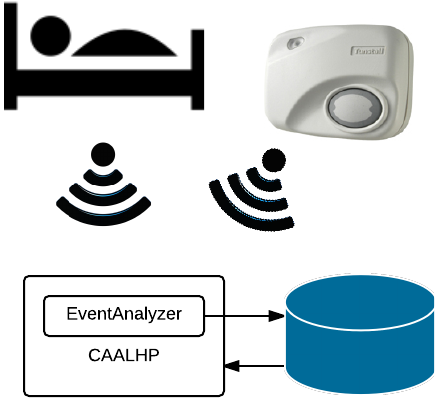
\includegraphics[width = 0.40 \textwidth]{Deployment}
	\caption{Deployment diagram of the system. 
		Each sensor is connected to the CAALHP with a wireless link.
		Inside the CAALHP runs the analyzer module with the False-positive filter in.}
	\label{fig:deployment}
\end{figure}

\begin{figure}[hbtp]
	\centering
	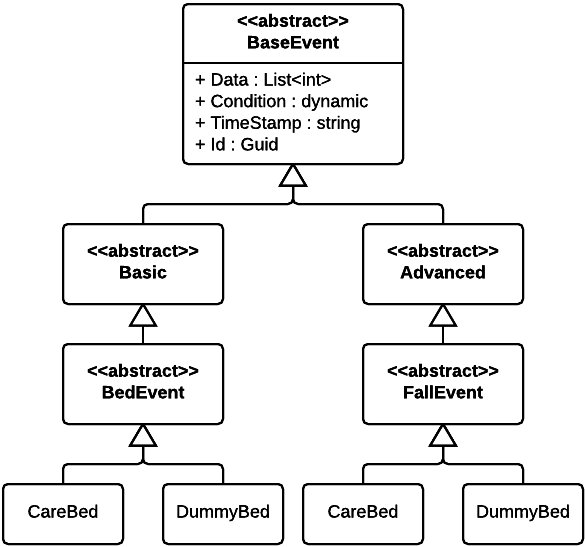
\includegraphics[width = 0.48 \textwidth]{UML}
	\caption{UML diagram of the event classes}
	\label{fig:UML}
\end{figure}


\vspace{-10pt}
\subsection{Evaluation}
\vspace{-15pt}

The program consist of 27 tests, all green, varying from unit testing inserting new elements in the databases, to integration testing calculations of new, incomming events and whether they are stored with correct values.

Besides that is several tests of activating the Shimmer unit tested, while sitting and not sitting in the Carebed, which all gives expected results of the likelyhood of the Shimmer being false-positive or not.



% Building a functional application requires a stable architecture.
% Building a scalable application requires a good architecture, which most of this project is capable of delivering.

% To analyze events, the events must comply as the same types of events\cite{BB-types}.
% Events all inherits from the same class, \texttt{BaseEvent}, which contains properties for data and probability of the event of occurrence.
% If the probability is not debatable (did or did not happen) an inherited class, \texttt{Basic}, converts the probability to a \texttt{bool} from a \texttt{dynamic}, or to probability in the \texttt{Advanced} class as an \texttt{int}.
% Because multiple manufacturers might produces sensors to do the exact same, e.g. register if you are in your bed, a general event for being in you bed is created. \texttt{BedEvent}, inheriting from \texttt{Basic}, allowing specific implementations to be made.
% Here a \texttt{DummyBed} and a \texttt{CareBed} (named by the product) is created inheriting from \texttt{BedEvent}.

% A fall detector bases its event on raw data.
% But since the data does not say either 'fall'/'not fall', it can give a probability of a fall.
% Letting a category of \texttt{FallEvent} inherit from \texttt{Advanced}, a \texttt{DummyFall} and a \texttt{ShimmerEvent} can send raw data as well as a probability to the CAALHP.

% When creating a service to analyze the events, each type of event it should be looking at must be registered.
% This will be done as soon as the class, \texttt{EventAnalyzer}, is initializing by creating new objects of each concrete class, which also will register them as possible entries for the MongoDB.
